\documentclass[compress]{beamer} %en animé
%\documentclass[trans]{beamer} %en superposé

%%%%%%%%%%%%%% LES PACKAGES
\input{les_packages_pour_beamer.tex}
%%%%%%%%%%%%%% THEME BEAMER
%votre nom court qui apparaîtra dans l'en tête
\newcommand{\initiales}{Yann Miquel--Erdmann }
\input{les_param_beamer_tipe}


%%%%%%%%%%%%%% MA PALETTE DE COULEURS
\input{la_palette.tex}
\definecolor{hellseahorse}{RGB}{204, 204, 255}
\definecolor{seahorse}{RGB}{204,180, 255}
\definecolor{darkseahorse}{RGB}{83, 74, 196}

%symboles pratiques
\newcommand{\flch}{\item[$\rightarrow$]}
\newcommand{\dc}{{\usebeamercolor[fg]{structure}$\hookrightarrow$}}
\newcommand{\ok}{\textcolor{vert}{\checkmark}}
\newcommand{\point}{{\usebeamercolor[fg]{structure}$\bullet\enskip$}}
\newcommand{\Point}{{\usebeamercolor[fg]{structure}$\bullet\enskip$}}


%styles
\newcommand{\couleur}[1]{{\usebeamercolor[fg]{structure}#1}}
\newcommand{\important}[1]{\couleur{\textbf{#1}}}
\newcommand{\remarque}[1]{\textit{\textrm{#1}}}

%pour le template
\newcommand{\lin}[1]{\mintinline{latex}{#1}}
%%%%%%%%%%%%%%%%%%%%%%%%%%%%%%%%%%%%%%%%%%%%%%%%%
\begin{document}
%

%%%%%%%%%%%%%%%%%%%%%%%%%%%%%%%%%%%%%%%%%%%%%%%%%
% A COMPLETER 
%%%%%%%%%%%%%%%%%%%%%%%%%%%%%%%%%%%%%%%%%%%%%%%%%

%entre crochet le titre court pour l'en tête puis le vrai titre
\title[La Transpilation]{
La transpilation de Fortran vers C
}

\author{
\large 
Présentation de \important{Yann MIQUEL--ERDMANN}\\[0.2cm]
Candidat n° \important{51280}\\[0.4cm]
\footnotesize
travail réalisé avec \couleur{Erwan FALAUX--BACHELOT}\\[0.4cm]
\vspace*{-1.2cm}
} 

%entre crochet la short date pour l'en-tête
\date[Juillet 2025]{}

\institute{}


%------------------------------------------------
\begin{frame}[plain]
\titlepage 
\addtocounter{framenumber}{-1} 
\end{frame}

%------------------------------------------------
\title[La transpilation de Fortran vers C]{}



\begin{frame}
    \frametitle{Introduction\esp}

    \vspace{0.5cm}
    \begin{minipage}[t]{0.48\textwidth}
        \includegraphics[scale=0.05]{static/Fortran_logo.svg.png}\\
        \textbf{Le Fortran:}\\ 
        Créé par:  John Backus, IBM\\
        Créé en:   1957\\
        Dernière version en: 2023\\
        Rang sur Github: $41^{\text{ème}}$
    \end{minipage}
    \hspace*{0.2cm}
    \begin{minipage}[t]{0.48\textwidth}
        \includegraphics[scale=0.05]{static/C_logo.png}\\
        \textbf{Le C:}\\
        Créé par: Dennis Ritchie et \\Kenneth Thompson, Bell Labs\\
        Créé en:  1972\\
        Dernière version en: 2024\\
        Rang sur Github: $9^{\text{ème}}$


    \end{minipage}
    
	\vspace*{2.9cm}

    \bandeauREF{%
        \hspace*{0.2cm}\textbf{Logo Fortran}: \url{https://commons.wikimedia.org/wiki/File:Fortran_logo.svg}\\
        \hspace*{0.2cm}\textbf{Logo C}: \url{https://commons.wikimedia.org/wiki/File:C_Logo.png}
    }

\end{frame}


\begin{frame}
    \frametitle{Problématique\esp}
    
    \begin{center}
        \textbf{Comment implémenter une conversion rapide de programmes Fortran en programmes C?}
    \end{center}

\end{frame}


\section{La transpilation}

\begin{frame}
<<<<<<< Updated upstream
<<<<<<< Updated upstream
    \frametitle{Définition}
    \input{tikz/FortranVersC.tex}
=======
=======
>>>>>>> Stashed changes
    \frametitle{Définition\esp}
    schéma avec un fichier Fortran, une machine et un fichier fortran
    et 
    programme fortran en entrée hello world et le programme obtenu en sortie 
>>>>>>> Stashed changes
\end{frame}


\begin{frame}
<<<<<<< Updated upstream
<<<<<<< Updated upstream

    \frametitle{Les étapes de la transpilation}

   \begin{tikzpicture}
  %placer les éléments
  \node[draw, rounded corners] (1) at (0,0) {Analyse lexicale Fortran};
  \node[draw, rounded corners] (2) [right=1cm of 1] {Analyse syntaxique Fortran};
  \node[fit=(1)(2), fill=briqueRouge, opacity=0.5, inner sep=0.1em, rounded corners] {};

  \node[draw,fill=vertdEau, rounded corners] (3) [right=1cm of 2] {Traduction Vers C};
  \node[draw,fill=vertdEau, rounded corners] (4) [above right =1cm of 2 ] {Traduction Vers Python};
  \node[draw,fill=vertdEau, rounded corners] (5) [below right =1cm of 2 ] {Traduction Vers Fortran};


  %les relier
  \draw[black, line width = 1pt, ->, >=latex] (1) -- (2);
  \draw[black, line width = 1pt, ->, >=latex] (2) -- (3);
  \draw[black, line width = 1pt, ->, >=latex] (2) -- (4);
  \draw[black, line width = 1pt, ->, >=latex] (2) -- (5);
  
\end{tikzpicture}

=======
=======
>>>>>>> Stashed changes
    \frametitle{\esp}
    parties d'un transpileur
    schéma tikz explication des différents paramètres (langage d'entrée et celui de sortie et le fait que ces langages sont constants pour le transpileur ) 
>>>>>>> Stashed changes
\end{frame}



\section{Analyse}

\subsection{Grammaire}
\begin{frame}
    \frametitle{Définition d'une grammaire\esp}

    \textbf{Grammaire non contextuelle:}
    \begin{minipage}[t]{0.7\textwidth}
        \vspace{-1.5em}
        \begin{align*}
            &\bullet\quad G = (\Sigma, V, P, S) \\
            &\bullet\quad \text{Les règles de production sont de la forme}\\
            & W \rightarrow U_1 \dots U_k \text{ avec } \forall i \in \llbracket 1, k \rrbracket,\ U_i \in V \cup \Sigma,\ W \in V \\
            \\[-2ex]
            &\Sigma = \{a,b\}, V = \{A,B\}, S = A, P = \{\\
            &\quad S \rightarrow A \\
            &\quad A \rightarrow aA \\
            &\quad A \rightarrow B \\
            &\quad B \rightarrow bB \\
            &\quad B \rightarrow \varepsilon \\
            &\}\\
            \\[-2ex]
            &\mathcal{L}(G) = a^* b^*
        \end{align*}
    \end{minipage}
    
\end{frame}

\begin{frame}
    \frametitle{Un exemple de grammaire\esp}
    \noindent
    \begin{tikzpicture}[remember picture, overlay]
    \node[anchor=south east, xshift=-1cm, yshift=2cm, ] at (current page.south east) {
        \begin{minipage}[b]{\linewidth}
        \inputminted[breaklines, fontsize=\smaller]{ocaml}{static/Grammaire_exemple.txt}
        \end{minipage}
    };
    \node<1>[anchor=south east, xshift=5cm] at (current page.south east) {
        \begin{minipage}[b]{\linewidth}
        \textbf{Types symbole OCaml}
        
        \inputminted[fontsize=\smaller]{ocaml}{static/type_symbol.ml}

        \end{minipage}
    };
    \node<2>[anchor=south east, xshift=5cm, yshift=0.38cm] at (current page.south east) {
        \begin{minipage}[b]{\linewidth}
        \textbf{Types grammaire OCaml}
        
        \inputminted[fontsize=\smaller]{ocaml}{static/type_grammaire.ml}

        \end{minipage}
    };



    \end{tikzpicture}
\end{frame}





\subsection{Analyse Lexicale}

\begin{frame}
    
    but: transformer le programme en entrée en une liste de lexèmes
    def lexème, bien faire la différence entre le lexème et le type reconnu, ie "Hello World" est un lexème de type string 

\end{frame}

\begin{frame}
    automates 
    automate tikz et curseurs 
    en vrai il y a 230 états
\end{frame}

\begin{frame}
    exemple de la liste de lexèmes qui est donnée en Ocaml pour notre programme

\end{frame}



\subsection{Analyse Syntaxique}

\begin{frame}
    \begin{tikzpicture}
    
    \tikzstyle{lien} = [->, >=latex]
    \tikzstyle{basic_text}=[text width=2cm, text badly centered]
    \tikzstyle{basic_node}=[draw = black,rounded corners=4pt, basic_text]
    \tikzstyle{wrapper}=[basic_node, inner sep=3pt]
    \tikzstyle{hidden}=[draw=black!0,color=black!0]
    \tikzstyle{faded}=[draw=black!20, color=black!20]
    

    \node [basic_node, text width=4cm, align=left] (Lexemes) {
        \scalebox{0.7}{
            \parbox{\textwidth}{

                \textbf{Liste de lexèmes}
                \inputminted{ocaml}{static/lexemes.ml}

            }
        }
    };


    \begin{scope}[shift={(6, 0)}]  
        \node [basic_node, text width=6cm, align=left] (AS) { 
            \scalebox{0.7}{
                \parbox{\textwidth}{
                    \textbf{Arbre de syntaxe}

                        
\tikzstyle{feuille}=[ draw, rectangle, inner sep = 0.12cm]
\tikzstyle{noeud}=[ draw, rectangle,rounded corners, minimum width= 0.64cm, line width = 1pt]
\begin{tikzpicture}[
        baseline=(base), 
        level/.style={sibling distance = 1.6cm/#1, level distance = 1cm},
        every node/.style={scale=0.6, font=\footnotesize}
    ]
    
    \node[ noeud] {Programme}
    child { 
        node[noeud] (base) {ProgramMC}
    }
    child {
        node[noeud] {NomProg}
        child {node[feuille] {"hello"}}
    }
    child [ level distance=2cm]{ 
        node [ noeud] {Print}
        child [sibling distance= 1cm] {
            node [noeud] {PrintMC}
        }
        child [sibling distance= 1cm]{
            node [noeud] {Asterisque}
        }
        child [sibling distance= 1cm]{
            node [noeud] {Virgule}
        }
        child [sibling distance= 1cm]{
            node [noeud] {Chaine}
            child { 
                node [feuille] {"Hello World"}
            }
        }
        child [sibling distance= 1cm] {
            node [noeud] {Paramliste}
            child { 
                node [feuille] {$\varepsilon$}
            }
        }
    }
    child { 
        node[ noeud] {EndProgramMC}
    }
    child {
        node[noeud] {NomProg}
        child {node[feuille] {"hello"}}
    };

\end{tikzpicture}
                }
            }
        };
    \end{scope}
    
 
    \draw [lien] (Lexemes.north) to[out=45, in=135]  node[midway, above] {\textbf{Analyse syntaxique}}   (AS.north west) ; 

\end{tikzpicture}
\end{frame}

\begin{frame}
    \frametitle{Algorithme LL1\esp}

    Nécessite:\\
    \vspace{0.05cm}\\{
    $\bullet$ Une grammaire LL (sans récursion gauche et sans ambigüité)\\
    $\text{\textcolor{red}{\ding{55}}} \ \ \mathcal{X} \rightarrow \mathcal{X}a$\\
    $\text{\textcolor{red}{\ding{55}}} \ \  \mathcal{X} \rightarrow a\mathcal{X}\mathcal{X} \ | \ \varepsilon  $\\}
    \vspace{0.25cm}\\
    {
    $\bullet$ LL1: un seul lexème suffit à choisir la règle de production\\
    $\mathcal{X} \rightarrow a\mathcal{X} | b\mathcal{X} $\\
    $\mathcal{Y} \rightarrow c\mathcal{Y} | d\mathcal{Y} $
}


\end{frame}

%%%%%%%%%%%%%%%% pas pour Erwan
\begin{frame}
    \frametitle{Tableau des premiers et suivants\esp}
    \small
    (1): Programme -> ProgramMC NomProgramme NouvelleLigne Print EndProgramMC NomProgramme\\
    (2): Print -> PrintMC Espace Asterisque Virgule Espace Chaine ParamListe\\
    (3): ParamListe -> Virgule Espace Chaine ParamListe\\
    (4): ParamListe ->  Epsilon \\

    \begin{tabular}{|c|c|c|}
    \hline
        & Premiers & Suivants\\  
    \hline
    Programme & $\{ProgramMC\}$ & $\{\$\}$ \\
    \hline
    Print & $\{PrintMC\}$ & $\{EndProgramMC\}$ \\
    \hline
    ParamListe & $\{ Virgule, \varepsilon \}$ & $\{EndProgramMC\}$\\
    \hline

    \end{tabular}

\end{frame}

\begin{frame}
    \frametitle{Tableau de lecture\esp}
    \small
    (1): Programme -> ProgramMC NomProgramme NouvelleLigne Print EndProgramMC NomProgramme\\
    (2): Print -> PrintMC Espace Asterisque Virgule Espace Chaine ParamListe\\
    (3): ParamListe -> Virgule Espace Chaine ParamListe\\
    (4): ParamListe ->  Epsilon \\\\
    \vspace{0.25cm}
    {
    \footnotesize
    \begin{tabular}{|c|c|c|c|c|c|c|c|c|c|}
        \hline
        & PrintMC & ProgramMC & EndProgramMC & Virgule \\
        \hline
        Programme & & 1 & & \\
        \hline
        Print & 2 & & & \\
        \hline
        ParamListe & & & 4 & 3 \\
        \hline
    \end{tabular}
    }

\end{frame}



\begin{frame}
    \frametitle{Arbre de syntaxe\esp}
    \begin{center}
        \scalebox{1.2}{
            
\tikzstyle{feuille}=[ draw, rectangle, inner sep = 0.12cm]
\tikzstyle{noeud}=[ draw, rectangle,rounded corners, minimum width= 0.64cm, line width = 1pt]
\begin{tikzpicture}[
        baseline=(base), 
        level/.style={sibling distance = 1.6cm/#1, level distance = 1cm},
        every node/.style={scale=0.6, font=\footnotesize}
    ]
    
    \node[ noeud] {Programme}
    child { 
        node[noeud] (base) {ProgramMC}
    }
    child {
        node[noeud] {NomProg}
        child {node[feuille] {"hello"}}
    }
    child [ level distance=2cm]{ 
        node [ noeud] {Print}
        child [sibling distance= 1cm] {
            node [noeud] {PrintMC}
        }
        child [sibling distance= 1cm]{
            node [noeud] {Asterisque}
        }
        child [sibling distance= 1cm]{
            node [noeud] {Virgule}
        }
        child [sibling distance= 1cm]{
            node [noeud] {Chaine}
            child { 
                node [feuille] {"Hello World"}
            }
        }
        child [sibling distance= 1cm] {
            node [noeud] {Paramliste}
            child { 
                node [feuille] {$\varepsilon$}
            }
        }
    }
    child { 
        node[ noeud] {EndProgramMC}
    }
    child {
        node[noeud] {NomProg}
        child {node[feuille] {"hello"}}
    };

\end{tikzpicture}
        }
        
    \end{center}
\end{frame}



\begin{frame}
    \frametitle{Conversion en arbre de syntaxe abstraite\esp}
    \begin{tikzpicture}
    
    \tikzstyle{lien} = [->, >=latex]
    \tikzstyle{basic_text}=[text width=2cm, text badly centered]
    \tikzstyle{basic_node}=[draw = black,rounded corners=4pt, basic_text]
    \tikzstyle{wrapper}=[basic_node, inner sep=3pt]
    \tikzstyle{hidden}=[draw=black!0,color=black!0]
    \tikzstyle{faded}=[draw=black!20, color=black!20]
    

    \node [basic_node, text width=6cm, align=left] (AS) {
         \scalebox{0.7}{
            \parbox{\textwidth}{
                    
\tikzstyle{feuille}=[ draw, rectangle, inner sep = 0.12cm]
\tikzstyle{noeud}=[ draw, rectangle,rounded corners, minimum width= 0.64cm, line width = 1pt]
\begin{tikzpicture}[
        baseline=(base), 
        level/.style={sibling distance = 1.6cm/#1, level distance = 1cm},
        every node/.style={scale=0.6, font=\footnotesize}
    ]
    
    \node[ noeud] {Programme}
    child { 
        node[noeud] (base) {ProgramMC}
    }
    child {
        node[noeud] {NomProg}
        child {node[feuille] {"hello"}}
    }
    child [ level distance=2cm]{ 
        node [ noeud] {Print}
        child [sibling distance= 1cm] {
            node [noeud] {PrintMC}
        }
        child [sibling distance= 1cm]{
            node [noeud] {Asterisque}
        }
        child [sibling distance= 1cm]{
            node [noeud] {Virgule}
        }
        child [sibling distance= 1cm]{
            node [noeud] {Chaine}
            child { 
                node [feuille] {"Hello World"}
            }
        }
        child [sibling distance= 1cm] {
            node [noeud] {Paramliste}
            child { 
                node [feuille] {$\varepsilon$}
            }
        }
    }
    child { 
        node[ noeud] {EndProgramMC}
    }
    child {
        node[noeud] {NomProg}
        child {node[feuille] {"hello"}}
    };

\end{tikzpicture}
            }
        }
    };

    \node [basic_node, text width=4cm, align=left] (AST) [right=1cm of AS] {
        \scalebox{0.7}{
            \parbox{\textwidth}{
                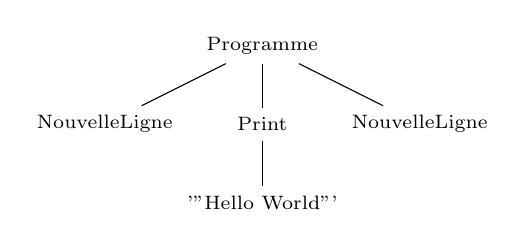
\begin{tikzpicture}
    \node[font=\scriptsize] (0) at (0, 0) {Programme};
    \node[font=\scriptsize] (1) at (-2, -1) {NouvelleLigne};
    \node[font=\scriptsize] (2) at (0, -1) {Print};
    \node[font=\scriptsize] (3) at (0, -2) {'"Hello World"'};
    \node[font=\scriptsize] (4) at (2, -1) {NouvelleLigne};
    
    \draw (0) -- (1);
    \draw (0) -- (2);
    \draw (2) -- (3);
    \draw (0) -- (4);
\end{tikzpicture}
            }
        }
    };
 
    \draw [lien] (AS.north) to[out=45, in=135]  node[midway, above] {\textbf{Conversion en arbre de syntaxe abstraite}}  (AST.north west) ; 

\end{tikzpicture}
\end{frame}



\section{Traduction}

\begin{frame}
    \frametitle{Traduction de l'arbre de syntaxe abstraite\esp}
    \begin{tikzpicture}
    
    \tikzstyle{lien} = [->, >=latex]
    \tikzstyle{basic_text}=[text width=2cm, text badly centered]
    \tikzstyle{basic_node}=[draw = black,rounded corners=4pt, basic_text]
    \tikzstyle{wrapper}=[basic_node, inner sep=3pt]
    \tikzstyle{hidden}=[draw=black!0,color=black!0]
    \tikzstyle{faded}=[draw=black!20, color=black!20]
    

    \node [basic_node, text width=4.7cm, align=left] (AST) {
         \scalebox{0.8}{
            \parbox{\textwidth}{
                \textbf{Arbre de syntaxe abstraite}
                \begin{tikzpicture}
    \node[font=\scriptsize] (0) at (0, 0) {Programme};
    \node[font=\scriptsize] (1) at (-2, -1) {NouvelleLigne};
    \node[font=\scriptsize] (2) at (0, -1) {Print};
    \node[font=\scriptsize] (3) at (0, -2) {'"Hello World"'};
    \node[font=\scriptsize] (4) at (2, -1) {NouvelleLigne};
    
    \draw (0) -- (1);
    \draw (0) -- (2);
    \draw (2) -- (3);
    \draw (0) -- (4);
\end{tikzpicture}
            }
        }
    };

    \node [basic_node, text width=5.3cm, align=left] (C) [right=1cm of AST] {
        \scalebox{0.9}{
            \parbox{\textwidth}{
                \textbf{Programme C}

                \inputminted[firstline=1, lastline=4,firstnumber=1]{c}{static/HelloWorld.c}
            } 
        } 
    };
 
    \draw [lien] (AST.north) to[out=45, in=135]  node[midway, above] {\textbf{Traduction en C}}  (C.north west) ; 

\end{tikzpicture}
\end{frame}

\section{Notre transpileur}

\begin{frame}
    \textbf{Notre transpileur peut:}\\
    $\bullet$ transpiler de Fortran vers C\\
    $\bullet$ transpiler de Fortran vers Fortran (formatage)\\
    \vspace{0.5cm} {
        \\
        Les variables, les assignations, les conditions, les boucles, les fonctions sont prises en charge par notre transpileur. 
    }   

\end{frame}


\begin{frame}
\noindent
\begin{minipage}[t]{0.48\textwidth}
    \scalebox{0.6}{
        \parbox{\textwidth}{
            \inputminted{fortran}{static/fibonacci.f90}
        }
    }
    
\end{minipage}
\hfill
\begin{minipage}[t]{0.48\textwidth}
    \scalebox{0.6}{
        \parbox{\textwidth}{
            \inputminted{c}{static/fibonacci.c}
        }
    }
\end{minipage}

\end{frame}


\section{Conclusion}


\begin{frame}
    \frametitle{Conclusion\esp}

    \point Conversion rapide\\
    \point Une partie du transpileur est construite automatiquement\\
    \point La syntaxe prise en charge est étendue\\
    \point Les parties du transpileur sont modulaires 

\end{frame}


\section{Annexe}

\foreach \name in{src/preprocessing/generateGrammar.ml, src/preprocessing/generateMlFiles.ml, src/prebuild/buildAutomaton.ml, src/abstractTokens.ml, src/bibliotheques.ml, src/environnement.ml, src/symbols.ml, src/traduction.ml, src/regex.ml, src/grammarFunctions.ml, src/grammar.ml, src/automates.ml, src/LL1.ml, src/convertToAbstract.ml, src/detAutomaton.ml, src/traductionC.ml, src/traductionFortran.ml, src/transpileurs.ml, src/main.ml}{
    \subsection{\name}
    \tiny   \inputminted[]{ocaml}{../../\name}
    
    \pagebreak
}




\end{document}
